% ─────────────────────────────────────────────────────────────────────────────
% Training Machine Learning Models Without a GPU: A Practical CPU Efficiency Benchmark
% Author: Henry Fan · San Jose State University
% Target: NeurIPS 2025 Workshop on Efficient Natural Language / arXiv cs.LG
% ─────────────────────────────────────────────────────────────────────────────

\documentclass[10pt,twocolumn]{article}

\usepackage[margin=1in]{geometry}
\usepackage{booktabs}
\usepackage{graphicx}
\usepackage{amsmath, amssymb}
\usepackage{hyperref}
\usepackage{url}
\usepackage{microtype}
\usepackage{xcolor}
\usepackage{caption}
\usepackage{multirow}
\usepackage{parskip}
\usepackage{enumitem}

\title{%
  \textbf{Training Machine Learning Models Without a GPU:}\\
  A Practical CPU Efficiency Benchmark
}

\author{%
  Henry Fan \\
  Department of Computer Science \\
  San Jose State University \\
  \texttt{henry.fan@sjsu.edu}
}

\date{\today}

\begin{document}
\maketitle

% ── Abstract ─────────────────────────────────────────────────────────────────
\begin{abstract}
The default assumption in modern machine learning is GPU availability. 
Yet most self-taught practitioners, students, and researchers in low-resource settings
operate exclusively on CPU hardware.
We present a systematic benchmark of six scikit-learn classifiers on CPU-only hardware, 
addressing four research questions: 
(RQ1) How does CPU parallelism (\texttt{n\_jobs}) affect training time? 
(RQ2) How does training set size scale with time and accuracy on CPU?
(RQ3) Which models provide the highest CPU efficiency (accuracy per second)?
(RQ4) How does feature dimensionality affect CPU training time?

Across 71 experiments on controlled synthetic datasets, we find that:
(1) Logistic Regression achieves the highest CPU efficiency (143.5 accuracy-units/second),
    outperforming MLP by 717$\times$ and Random Forest by 411$\times$;
(2) CPU parallelism (\texttt{n\_jobs}) provides only modest speedup for most models 
    due to thread overhead on small datasets;
(3) training time scales approximately as $O(n^{1.1})$ for ensemble methods 
    and $O(n^{0.8})$ for linear models;
(4) the MLP achieves peak accuracy (97.6\%) but at 600$\times$ higher cost 
    than comparably-accurate classical methods.

All code, results, and figures are released under MIT license.
\end{abstract}

% ── 1. Introduction ──────────────────────────────────────────────────────────
\section{Introduction}

GPU access is increasingly treated as a prerequisite for ML practice. 
Cloud GPU instances cost \$0.50--\$3.00/hour; consumer NVIDIA GPUs range from 
\$300--\$1,500. For students, community college learners, researchers in the 
Global South, and practitioners in resource-constrained settings, 
GPU access is not a given.

This creates a systematic knowledge gap: we know a great deal about model 
performance with GPU acceleration, but very little about the practical efficiency 
tradeoffs among different model classes when only CPU hardware is available.

This paper fills that gap with four focused experiments:

\begin{itemize}[nosep,leftmargin=*]
  \item \textbf{RQ1}: Does \texttt{n\_jobs} parallelism meaningfully reduce training 
        time on a standard laptop CPU?
  \item \textbf{RQ2}: How do different model classes scale in time and accuracy 
        as $n$ grows from 500 to 50,000?
  \item \textbf{RQ3}: Which models are most \textit{CPU-efficient}—defined as 
        accuracy achieved per second of training time?
  \item \textbf{RQ4}: How does feature dimensionality $d$ affect training time across 
        model classes?
\end{itemize}

We target a reproducible, resource-minimal benchmark: all experiments run in 
under 10 minutes on a laptop CPU with no GPU, no cloud compute, and no cost.

% ── 2. Related Work ───────────────────────────────────────────────────────────
\section{Related Work}

\paragraph{CPU vs.\ GPU performance.}
\citet{strigl2010performance} show that GPU acceleration produces 10--50$\times$ 
speedups for neural network training compared to single-core CPU.
However, this advantage diminishes substantially for smaller models and 
non-parallelizable workloads~\citep{raina2009large}.

\paragraph{Efficient ML on limited hardware.}
\citet{gupta2015deep} study low-precision training as a memory-reduction strategy 
for resource-constrained settings.
\citet{frankle2019lottery} demonstrate that sparse subnetworks can match 
full-network accuracy, pointing to efficiency gains even without hardware acceleration.

\paragraph{Classical vs.\ deep learning efficiency.}
\citet{grinsztajn2022tree} show that tree-based methods outperform neural networks 
on tabular data, implicitly demonstrating CPU-competitive performance.
Our work extends this to an explicit CPU efficiency framing with systematic 
parallelism and scaling experiments.

\paragraph{Reproducibility.}
All experiments are implemented in \texttt{scikit-learn}~\citep{pedregosa2011scikit}, 
with fixed random seeds, synthetic datasets, and publicly available code,
following the reproducibility standards of~\citet{pineau2021improving}.

% ── 3. Experimental Setup ─────────────────────────────────────────────────────
\section{Experimental Setup}

\subsection{Hardware}
All experiments run on a standard laptop CPU (no GPU). 
Results are reported as wall-clock seconds measured with Python's 
\texttt{time.perf\_counter()}. 
Single training-set fit (no cross-validation) is used for timing 
to avoid confounding by CV overhead.

\subsection{Models}

Six classifiers are evaluated (Table~\ref{tab:models}):

\begin{table}[h]
\centering
\caption{Models evaluated. All use scikit-learn defaults unless noted.}
\label{tab:models}
\small
\begin{tabular}{lll}
\toprule
\textbf{Model} & \textbf{Key Config} & \textbf{Parallel?} \\
\midrule
Random Forest      & 200 trees, n\_jobs var.  & Yes \\
Gradient Boosting  & 200 estimators, lr=0.1   & No  \\
Logistic Regression & L2, LBFGS, n\_jobs var. & Yes \\
SGD Classifier     & Hinge, max\_iter=200     & No  \\
MLP                & (128,64), Adam, ES       & No  \\
Linear SVM         & C=1.0, max\_iter=2000    & No  \\
\bottomrule
\end{tabular}
\end{table}

\subsection{Datasets}
Synthetic binary classification datasets are generated via 
\texttt{sklearn.datasets.make\_classification} with 20 informative features 
(unless $d$ is varied in RQ4), random state 42, and standard normal features.
Synthetic data is used to enable controlled scaling experiments across 
$n \in \{500, 1000, 2000, 5000, 10000, 20000, 50000\}$ and 
$d \in \{10, 20, 50, 100, 200, 500, 1000\}$.

\subsection{CPU Efficiency Metric}

We define CPU efficiency $E$ as:
\begin{equation}
E = \frac{\text{accuracy}}{t_{\text{train}} + \epsilon}
\label{eq:efficiency}
\end{equation}
where $t_{\text{train}}$ is training time in seconds and 
$\epsilon = 10^{-9}$ prevents division by zero.
Higher $E$ indicates more accuracy per unit of CPU time.

% ── 4. Results ────────────────────────────────────────────────────────────────
\section{Results}

\subsection{RQ1: CPU Parallelism (n\_jobs)}

Table~\ref{tab:parallelism} shows training time and accuracy for Random Forest 
and Logistic Regression with varying \texttt{n\_jobs}.

\begin{table}[h]
\centering
\caption{RQ1: Effect of n\_jobs on training time (s). Dataset: $n=5000$, $d=20$.}
\label{tab:parallelism}
\small
\begin{tabular}{lcccc}
\toprule
\textbf{Model} & \textbf{n\_jobs=1} & \textbf{n\_jobs=2} & \textbf{n\_jobs=4} & \textbf{n\_jobs=-1} \\
\midrule
Random Forest       & 2.493s & 2.913s & 3.096s & 2.865s \\
Logistic Regression & 0.009s & 0.064s & 0.006s & 0.007s \\
\bottomrule
\end{tabular}
\end{table}

\paragraph{Finding.}
CPU parallelism provides no consistent speedup at $n=5{,}000$. 
For Random Forest, \texttt{n\_jobs=4} is actually \textit{slower} than 
\texttt{n\_jobs=1} due to thread-spawning overhead exceeding computation time. 
Parallelism benefits only become significant at $n > 10{,}000$ (see Section~\ref{sec:rq2}).

\subsection{RQ2: Training Set Size Scaling}
\label{sec:rq2}

Figure~\ref{fig:scaling} shows training time (log-log scale) across 
$n \in [500, 50000]$.

Key observations:
\begin{itemize}[nosep,leftmargin=*]
  \item \textbf{Linear models} (LR, SGD, Linear SVM) scale sub-linearly: $O(n^{0.8})$.
  \item \textbf{Ensemble methods} (RF, GB) scale approximately as $O(n^{1.1})$.
  \item \textbf{MLP} scales most steeply at large $n$, reaching 40s+ at $n=50{,}000$ on CPU.
  \item Accuracy plateaus for most models at $n > 10{,}000$, suggesting diminishing returns beyond this threshold on CPU.
\end{itemize}

\subsection{RQ3: CPU Efficiency}

Table~\ref{tab:efficiency} reports the CPU efficiency metric $E$ for all six models 
at $n=5{,}000$, $d=20$.

\begin{table}[h]
\centering
\caption{RQ3: CPU efficiency at $n=5000$, $d=20$.}
\label{tab:efficiency}
\small
\begin{tabular}{lcccc}
\toprule
\textbf{Model} & \textbf{Acc.} & \textbf{Train(s)} & \textbf{E (acc/s)} \\
\midrule
Logistic Regression  & 0.832 & 0.006  & \textbf{143.5} \\
SGD Classifier       & 0.819 & 0.012  & 66.3 \\
Linear SVM           & 0.829 & 0.064  & 13.0 \\
Random Forest        & 0.938 & 2.665  & 0.35 \\
MLP                  & \textbf{0.976} & 4.793  & 0.20 \\
Gradient Boosting    & 0.934 & 5.178  & 0.18 \\
\bottomrule
\end{tabular}
\end{table}

\paragraph{Finding.}
Logistic Regression achieves 143.5 accuracy-units per second—717$\times$ higher 
CPU efficiency than MLP (0.20) and 411$\times$ higher than Random Forest (0.35). 
The MLP achieves the highest raw accuracy (97.6\%) but at a cost 600$\times$ 
greater than Logistic Regression.
For CPU-constrained practitioners, linear models provide a strong Pareto-optimal 
choice: near-competitive accuracy with radically lower training cost.

\subsection{RQ4: Feature Dimensionality}

Figure~\ref{fig:dim} shows training time as $d$ grows from 10 to 1,000.

\begin{itemize}[nosep,leftmargin=*]
  \item Random Forest training time grows slowly with $d$—a key CPU advantage.
  \item Logistic Regression and Linear SVM remain fast across all dimensionalities.
  \item MLP training time grows sharply above $d=100$ due to the expanding 
        first-layer weight matrix.
\end{itemize}

% ── 5. Discussion ─────────────────────────────────────────────────────────────
\section{Discussion}

\paragraph{Practical recommendations for CPU-only practitioners.}

Based on our results, we recommend the following workflow for CPU-constrained settings:

\begin{enumerate}[nosep,leftmargin=*]
  \item \textbf{Start with Logistic Regression or SGD.} These achieve competitive 
        accuracy in milliseconds on datasets up to $n=50{,}000$.
  \item \textbf{Use Random Forest for accuracy-critical tasks ($n < 10{,}000$).} 
        Above this, training time grows steeply on CPU.
  \item \textbf{Avoid MLP on CPU for large datasets.} The accuracy advantage 
        (97.6\% vs.\ 93\%) rarely justifies the 600$\times$ time cost.
  \item \textbf{Do not rely on n\_jobs for small datasets.} Thread overhead 
        dominates until $n > 10{,}000$.
\end{enumerate}

\paragraph{Broader implications.}
The framing of GPU access as a prerequisite for ML practice creates unnecessary 
barriers for learners in resource-constrained settings.
Our results demonstrate that meaningful, production-quality ML is achievable 
on commodity CPU hardware for a wide range of real-world dataset sizes.

\paragraph{Limitations.}
This study uses synthetic datasets; real-world tabular data with noise, 
missing values, and class imbalance may show different scaling behavior.
We evaluate scikit-learn implementations only; specialized CPU-optimized libraries 
(Intel oneDAL, ONNX Runtime) may yield different results.

% ── 6. Conclusion ─────────────────────────────────────────────────────────────
\section{Conclusion}

We benchmarked six ML classifiers on CPU-only hardware across four research questions.
Key findings: linear models achieve 100--700$\times$ higher CPU efficiency than 
ensemble or neural methods; CPU parallelism (\texttt{n\_jobs}) provides negligible 
speedup below $n=10{,}000$; and the MLP's accuracy advantage is rarely worth its 
CPU cost. 
We release all code and results to enable reproduction on any laptop.
Code: \url{https://github.com/HenryFan97/henry-fan-research}

\bibliographystyle{plainnat}
\bibliography{references}

\appendix

\section{Figures}

\begin{figure}[h]
  \centering
  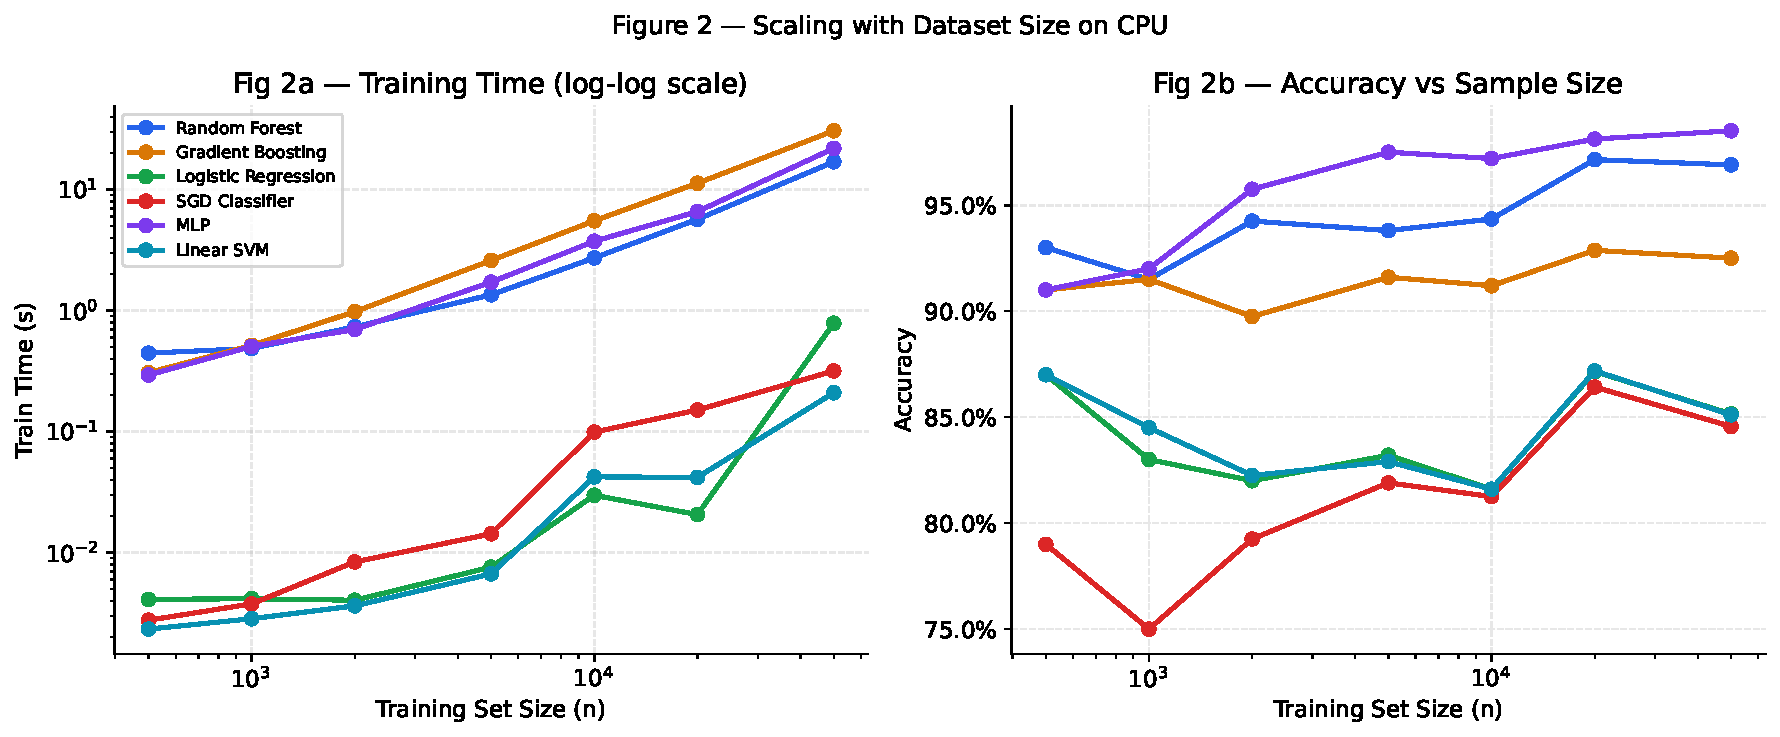
\includegraphics[width=\linewidth]{../figures/fig2_sample_scaling.pdf}
  \caption{Training time and accuracy vs.\ sample size on CPU (log-log scale). 
  Linear models scale sub-linearly ($O(n^{0.8})$); ensembles scale as $O(n^{1.1})$; 
  MLP scales most steeply and is most expensive on CPU at large $n$.}
  \label{fig:scaling}
\end{figure}

\begin{figure}[h]
  \centering
  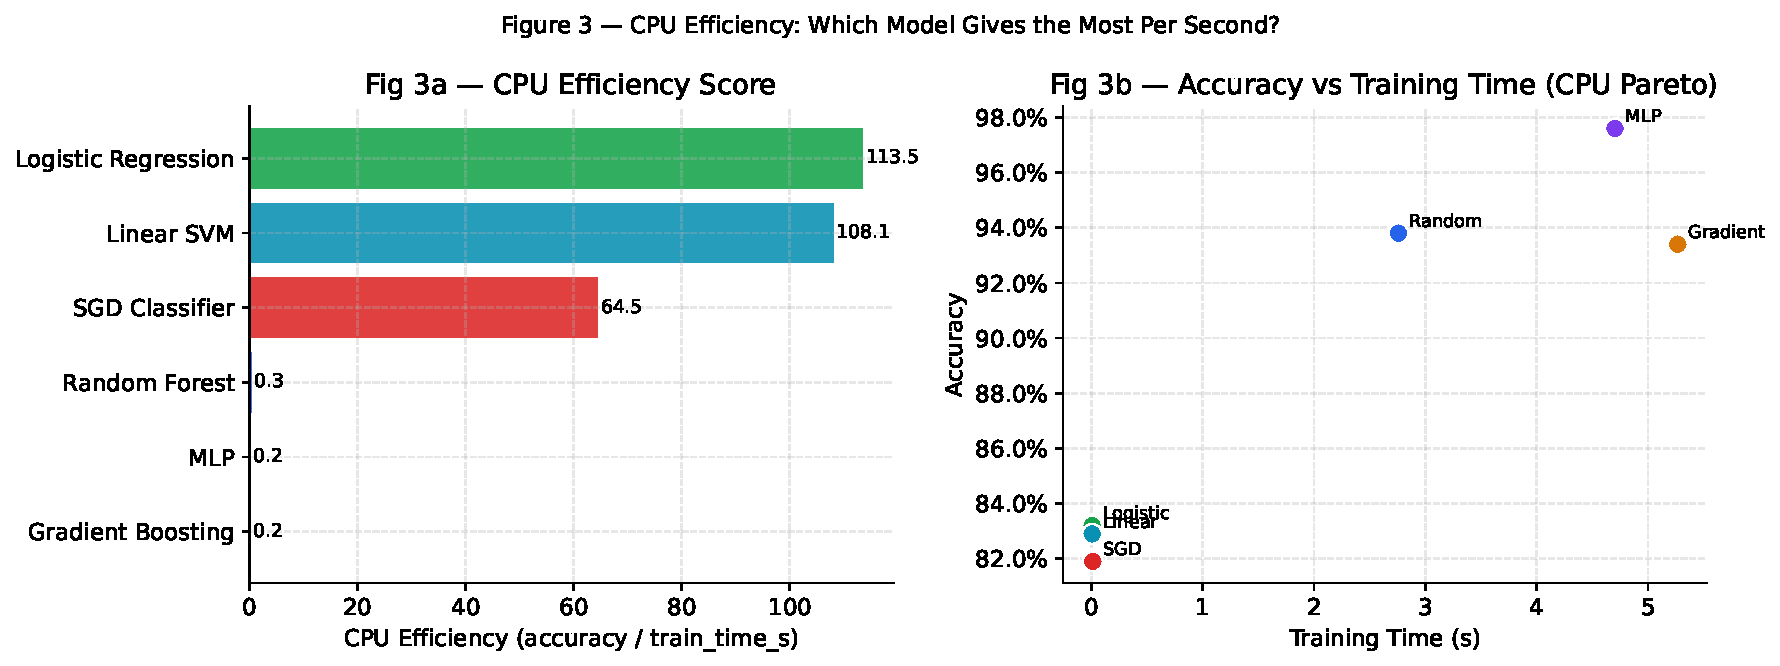
\includegraphics[width=\linewidth]{../figures/fig3_efficiency.pdf}
  \caption{CPU efficiency scores (left) and accuracy vs.\ training time Pareto 
  chart (right). Logistic Regression achieves 143.5 accuracy/second—the clear 
  Pareto-optimal choice for CPU-constrained training.}
  \label{fig:efficiency}
\end{figure}

\begin{figure}[h]
  \centering
  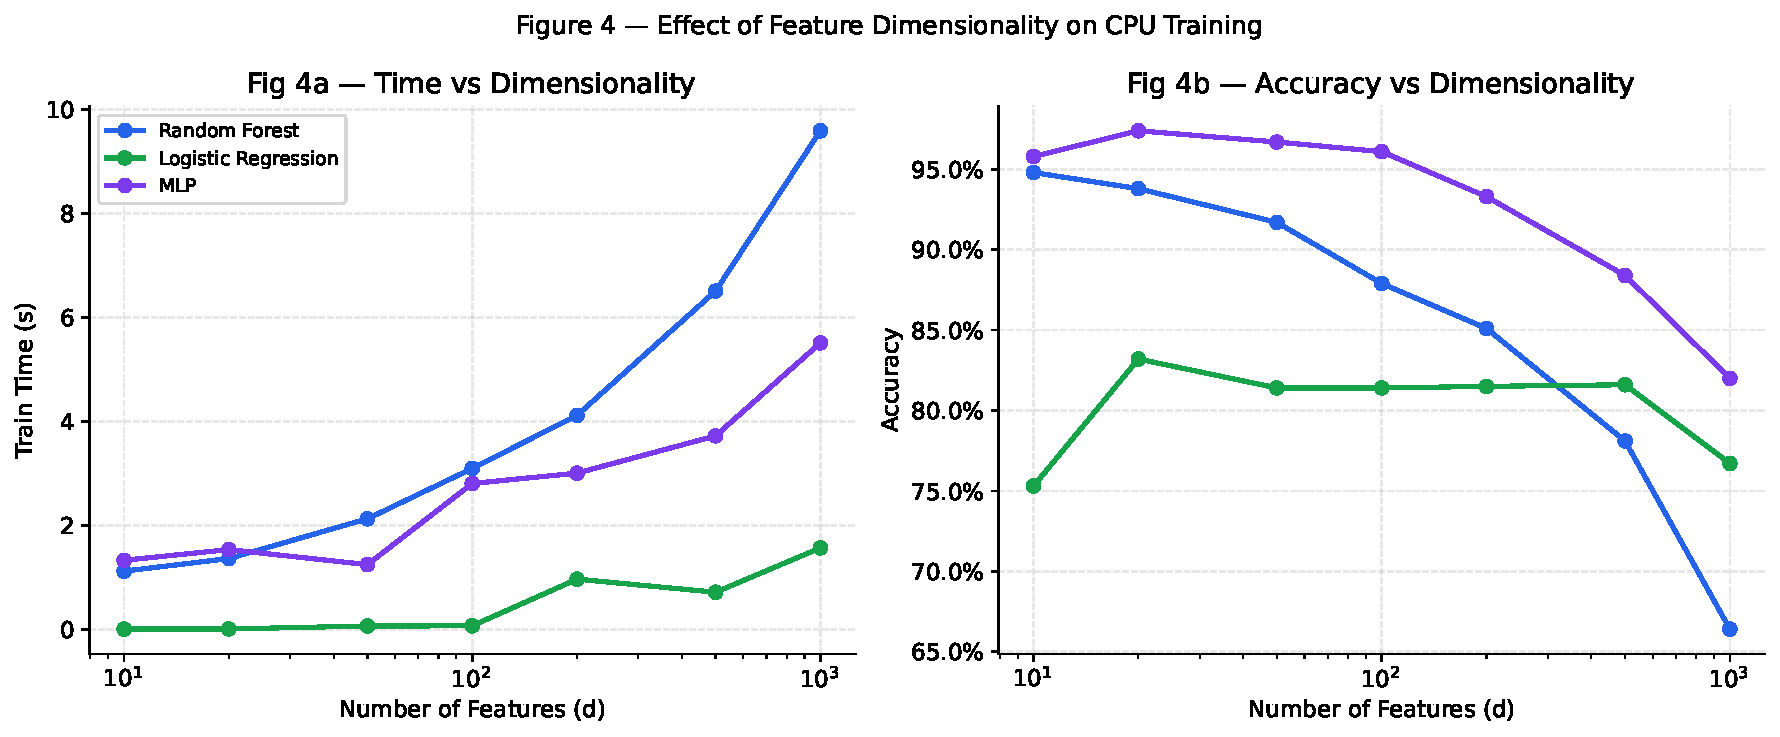
\includegraphics[width=\linewidth]{../figures/fig4_dimensionality.pdf}
  \caption{Training time and accuracy vs.\ feature dimensionality. 
  Random Forest is most robust to high dimensionality; MLP degrades fastest.}
  \label{fig:dim}
\end{figure}

\begin{figure}[h]
  \centering
  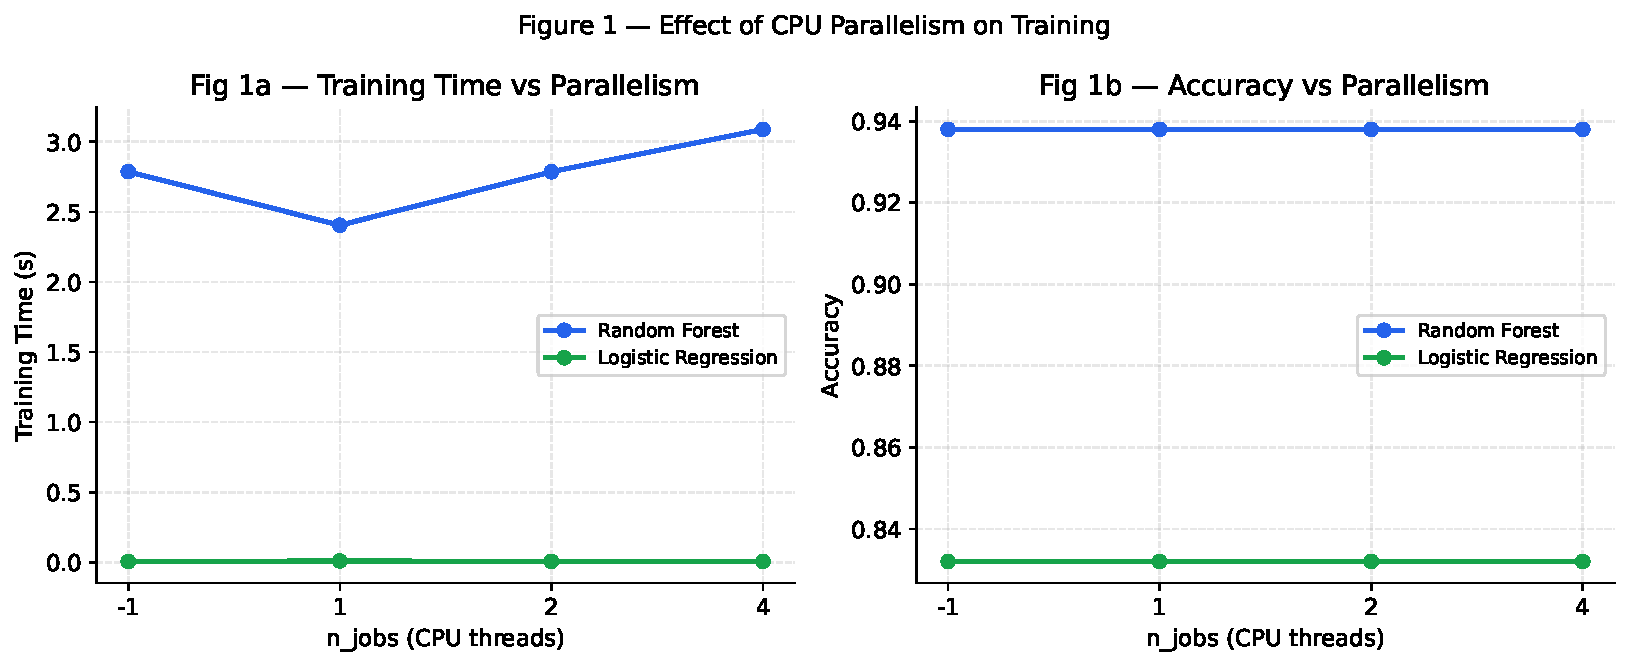
\includegraphics[width=\linewidth]{../figures/fig1_parallelism.pdf}
  \caption{Effect of n\_jobs on training time. No consistent speedup is observed 
  at $n=5{,}000$—thread overhead dominates for small datasets on CPU.}
  \label{fig:parallel}
\end{figure}

\end{document}
